\documentclass[1p]{elsarticle_modified}
%\bibliographystyle{elsarticle-num}

%\usepackage[colorlinks]{hyperref}
%\usepackage{abbrmath_seonhwa} %\Abb, \Ascr, \Acal ,\Abf, \Afrak
\usepackage{amsfonts}
\usepackage{amssymb}
\usepackage{amsmath}
\usepackage{amsthm}
\usepackage{scalefnt}
\usepackage{amsbsy}
\usepackage{kotex}
\usepackage{caption}
\usepackage{subfig}
\usepackage{color}
\usepackage{graphicx}
\usepackage{xcolor} %% white, black, red, green, blue, cyan, magenta, yellow
\usepackage{float}
\usepackage{setspace}
\usepackage{hyperref}

\usepackage{tikz}
\usetikzlibrary{arrows}

\usepackage{multirow}
\usepackage{array} % fixed length table
\usepackage{hhline}

%%%%%%%%%%%%%%%%%%%%%
\makeatletter
\renewcommand*\env@matrix[1][\arraystretch]{%
	\edef\arraystretch{#1}%
	\hskip -\arraycolsep
	\let\@ifnextchar\new@ifnextchar
	\array{*\c@MaxMatrixCols c}}
\makeatother %https://tex.stackexchange.com/questions/14071/how-can-i-increase-the-line-spacing-in-a-matrix
%%%%%%%%%%%%%%%

\usepackage[normalem]{ulem}

\newcommand{\msout}[1]{\ifmmode\text{\sout{\ensuremath{#1}}}\else\sout{#1}\fi}
%SOURCE: \msout is \stkout macro in https://tex.stackexchange.com/questions/20609/strikeout-in-math-mode

\newcommand{\cancel}[1]{
	\ifmmode
	{\color{red}\msout{#1}}
	\else
	{\color{red}\sout{#1}}
	\fi
}

\newcommand{\add}[1]{
	{\color{blue}\uwave{#1}}
}

\newcommand{\replace}[2]{
	\ifmmode
	{\color{red}\msout{#1}}{\color{blue}\uwave{#2}}
	\else
	{\color{red}\sout{#1}}{\color{blue}\uwave{#2}}
	\fi
}

\newcommand{\Sol}{\mathcal{S}} %segment
\newcommand{\D}{D} %diagram
\newcommand{\A}{\mathcal{A}} %arc


%%%%%%%%%%%%%%%%%%%%%%%%%%%%%5 test

\def\sl{\operatorname{\textup{SL}}(2,\Cbb)}
\def\psl{\operatorname{\textup{PSL}}(2,\Cbb)}
\def\quan{\mkern 1mu \triangleright \mkern 1mu}

\theoremstyle{definition}
\newtheorem{thm}{Theorem}[section]
\newtheorem{prop}[thm]{Proposition}
\newtheorem{lem}[thm]{Lemma}
\newtheorem{ques}[thm]{Question}
\newtheorem{cor}[thm]{Corollary}
\newtheorem{defn}[thm]{Definition}
\newtheorem{exam}[thm]{Example}
\newtheorem{rmk}[thm]{Remark}
\newtheorem{alg}[thm]{Algorithm}

\newcommand{\I}{\sqrt{-1}}
\begin{document}

%\begin{frontmatter}
%
%\title{Boundary parabolic representations of knots up to 8 crossings}
%
%%% Group authors per affiliation:
%\author{Yunhi Cho} 
%\address{Department of Mathematics, University of Seoul, Seoul, Korea}
%\ead{yhcho@uos.ac.kr}
%
%
%\author{Seonhwa Kim} %\fnref{s_kim}}
%\address{Center for Geometry and Physics, Institute for Basic Science, Pohang, 37673, Korea}
%\ead{ryeona17@ibs.re.kr}
%
%\author{Hyuk Kim}
%\address{Department of Mathematical Sciences, Seoul National University, Seoul 08826, Korea}
%\ead{hyukkim@snu.ac.kr}
%
%\author{Seokbeom Yoon}
%\address{Department of Mathematical Sciences, Seoul National University, Seoul, 08826,  Korea}
%\ead{sbyoon15@snu.ac.kr}
%
%\begin{abstract}
%We find all boundary parabolic representation of knots up to 8 crossings.
%
%\end{abstract}
%\begin{keyword}
%    \MSC[2010] 57M25 
%\end{keyword}
%
%\end{frontmatter}

%\linenumbers
%\tableofcontents
%
\newcommand\colored[1]{\textcolor{white}{\rule[-0.35ex]{0.8em}{1.4ex}}\kern-0.8em\color{red} #1}%
%\newcommand\colored[1]{\textcolor{white}{ #1}\kern-2.17ex	\textcolor{white}{ #1}\kern-1.81ex	\textcolor{white}{ #1}\kern-2.15ex\color{red}#1	}

{\Large $\underline{11a_{116}~(K11a_{116})}$}

\setlength{\tabcolsep}{10pt}
\renewcommand{\arraystretch}{1.6}
\vspace{1cm}\begin{tabular}{m{100pt}>{\centering\arraybackslash}m{274pt}}
\multirow{5}{120pt}{
	\centering
	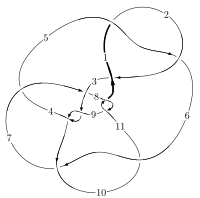
\includegraphics[width=112pt]{../../../GIT/diagram.site/Diagrams/png/365_11a_116.png}\\
\ \ \ A knot diagram\footnotemark}&
\allowdisplaybreaks
\textbf{Linearized knot diagam} \\
\cline{2-2}
 &
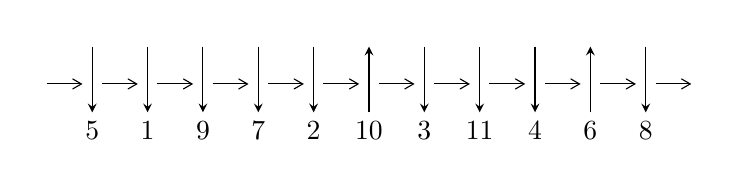
\begin{tikzpicture}[x=20pt, y=17pt]
	% nodes
	\node (C0) at (0, 0) {};
	\node (C1) at (1, 0) {};
	\node (C1U) at (1, +1) {};
	\node (C1D) at (1, -1) {5};

	\node (C2) at (2, 0) {};
	\node (C2U) at (2, +1) {};
	\node (C2D) at (2, -1) {1};

	\node (C3) at (3, 0) {};
	\node (C3U) at (3, +1) {};
	\node (C3D) at (3, -1) {9};

	\node (C4) at (4, 0) {};
	\node (C4U) at (4, +1) {};
	\node (C4D) at (4, -1) {7};

	\node (C5) at (5, 0) {};
	\node (C5U) at (5, +1) {};
	\node (C5D) at (5, -1) {2};

	\node (C6) at (6, 0) {};
	\node (C6U) at (6, +1) {};
	\node (C6D) at (6, -1) {10};

	\node (C7) at (7, 0) {};
	\node (C7U) at (7, +1) {};
	\node (C7D) at (7, -1) {3};

	\node (C8) at (8, 0) {};
	\node (C8U) at (8, +1) {};
	\node (C8D) at (8, -1) {11};

	\node (C9) at (9, 0) {};
	\node (C9U) at (9, +1) {};
	\node (C9D) at (9, -1) {4};

	\node (C10) at (10, 0) {};
	\node (C10U) at (10, +1) {};
	\node (C10D) at (10, -1) {6};

	\node (C11) at (11, 0) {};
	\node (C11U) at (11, +1) {};
	\node (C11D) at (11, -1) {8};
	\node (C12) at (12, 0) {};

	% arrows
	\draw[->,>={angle 60}]
	(C0) edge (C1) (C1) edge (C2) (C2) edge (C3) (C3) edge (C4) (C4) edge (C5) (C5) edge (C6) (C6) edge (C7) (C7) edge (C8) (C8) edge (C9) (C9) edge (C10) (C10) edge (C11) (C11) edge (C12) ;	\draw[->,>=stealth]
	(C1U) edge (C1D) (C2U) edge (C2D) (C3U) edge (C3D) (C4U) edge (C4D) (C5U) edge (C5D) (C6D) edge (C6U) (C7U) edge (C7D) (C8U) edge (C8D) (C9U) edge (C9D) (C10D) edge (C10U) (C11U) edge (C11D) ;
	\end{tikzpicture} \\
\hhline{~~} \\& 
\textbf{Solving Sequence} \\ \cline{2-2} 
 &
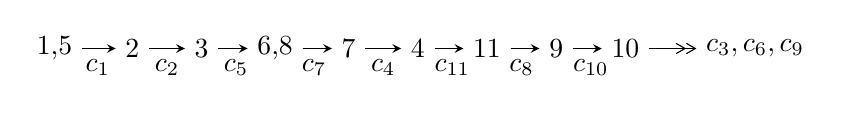
\begin{tikzpicture}[x=25pt, y=7pt]
	% node
	\node (A0) at (-1/8, 0) {1,5};
	\node (A1) at (1, 0) {2};
	\node (A2) at (2, 0) {3};
	\node (A3) at (49/16, 0) {6,8};
	\node (A4) at (33/8, 0) {7};
	\node (A5) at (41/8, 0) {4};
	\node (A6) at (49/8, 0) {11};
	\node (A7) at (57/8, 0) {9};
	\node (A8) at (65/8, 0) {10};
	\node (C1) at (1/2, -1) {$c_{1}$};
	\node (C2) at (3/2, -1) {$c_{2}$};
	\node (C3) at (5/2, -1) {$c_{5}$};
	\node (C4) at (29/8, -1) {$c_{7}$};
	\node (C5) at (37/8, -1) {$c_{4}$};
	\node (C6) at (45/8, -1) {$c_{11}$};
	\node (C7) at (53/8, -1) {$c_{8}$};
	\node (C8) at (61/8, -1) {$c_{10}$};
	\node (A9) at (10, 0) {$c_{3},c_{6},c_{9}$};

	% edge
	\draw[->,>=stealth]	
	(A0) edge (A1) (A1) edge (A2) (A2) edge (A3) (A3) edge (A4) (A4) edge (A5) (A5) edge (A6) (A6) edge (A7) (A7) edge (A8) ;
	\draw[->>,>={angle 60}]	
	(A8) edge (A9);
\end{tikzpicture} \\ 

\end{tabular} \\

\footnotetext{
The image of knot diagram is generated by the software ``\textbf{Draw programme}" developed by Andrew Bartholomew(\url{http://www.layer8.co.uk/maths/draw/index.htm\#Running-draw}), where we modified some parts for our purpose(\url{https://github.com/CATsTAILs/LinksPainter}).
}\phantom \\ \newline 
\centering \textbf{Ideals for irreducible components\footnotemark of $X_{\text{par}}$} 
 
\begin{align*}
I^u_{1}&=\langle 
3.00006\times10^{116} u^{83}-6.80069\times10^{116} u^{82}+\cdots+1.41969\times10^{116} b-5.82904\times10^{117},\\
\phantom{I^u_{1}}&\phantom{= \langle  }-2.28133\times10^{118} u^{83}+8.84656\times10^{118} u^{82}+\cdots+2.41347\times10^{117} a-2.50578\times10^{119},\\
\phantom{I^u_{1}}&\phantom{= \langle  }u^{84}-5 u^{83}+\cdots+84 u-17\rangle \\
I^u_{2}&=\langle 
- u^{15}+4 u^{13}- u^{12}-10 u^{11}+4 u^{10}+15 u^9-10 u^8-18 u^7+12 u^6+13 u^5-11 u^4-6 u^3+7 u^2+b+2 u-2,\\
\phantom{I^u_{2}}&\phantom{= \langle  }-4 u^{15}+2 u^{14}+\cdots+a-3,\;u^{16}-4 u^{14}+10 u^{12}-16 u^{10}+u^9+21 u^8-19 u^6-2 u^5+11 u^4+u^3-4 u^2+1\rangle \\
\\
\end{align*}
\raggedright * 2 irreducible components of $\dim_{\mathbb{C}}=0$, with total 100 representations.\\
\footnotetext{All coefficients of polynomials are rational numbers. But the coefficients are sometimes approximated in decimal forms when there is not enough margin.}
\newpage
\renewcommand{\arraystretch}{1}
\centering \section*{I. $I^u_{1}= \langle 3.00\times10^{116} u^{83}-6.80\times10^{116} u^{82}+\cdots+1.42\times10^{116} b-5.83\times10^{117},\;-2.28\times10^{118} u^{83}+8.85\times10^{118} u^{82}+\cdots+2.41\times10^{117} a-2.51\times10^{119},\;u^{84}-5 u^{83}+\cdots+84 u-17 \rangle$}
\flushleft \textbf{(i) Arc colorings}\\
\begin{tabular}{m{7pt} m{180pt} m{7pt} m{180pt} }
\flushright $a_{1}=$&$\begin{pmatrix}1\\0\end{pmatrix}$ \\
\flushright $a_{5}=$&$\begin{pmatrix}0\\u\end{pmatrix}$ \\
\flushright $a_{2}=$&$\begin{pmatrix}1\\u^2\end{pmatrix}$ \\
\flushright $a_{3}=$&$\begin{pmatrix}- u^2+1\\u^2\end{pmatrix}$ \\
\flushright $a_{6}=$&$\begin{pmatrix}- u\\- u^3+u\end{pmatrix}$ \\
\flushright $a_{8}=$&$\begin{pmatrix}9.45248 u^{83}-36.6550 u^{82}+\cdots-485.532 u+103.825\\-2.11318 u^{83}+4.79027 u^{82}+\cdots-94.7799 u+41.0586\end{pmatrix}$ \\
\flushright $a_{7}=$&$\begin{pmatrix}7.48664 u^{83}-30.4435 u^{82}+\cdots-470.700 u+107.907\\-3.18690 u^{83}+11.1199 u^{82}+\cdots+76.7100 u-4.10517\end{pmatrix}$ \\
\flushright $a_{4}=$&$\begin{pmatrix}2.35529 u^{83}-10.5702 u^{82}+\cdots-179.463 u+31.5654\\-6.32184 u^{83}+25.6009 u^{82}+\cdots+384.645 u-88.1719\end{pmatrix}$ \\
\flushright $a_{11}=$&$\begin{pmatrix}-2.19228 u^{83}+8.56750 u^{82}+\cdots+103.363 u-13.1483\\2.18637 u^{83}-10.0740 u^{82}+\cdots-193.104 u+50.8633\end{pmatrix}$ \\
\flushright $a_{9}=$&$\begin{pmatrix}-5.09729 u^{83}+19.6966 u^{82}+\cdots+234.342 u-37.5811\\1.58854 u^{83}-2.48611 u^{82}+\cdots+94.3251 u-33.4791\end{pmatrix}$ \\
\flushright $a_{10}=$&$\begin{pmatrix}1.48871 u^{83}-5.29073 u^{82}+\cdots-48.2350 u+12.4535\\2.48559 u^{83}-14.1259 u^{82}+\cdots-360.853 u+102.556\end{pmatrix}$\\ \flushright $a_{10}=$&$\begin{pmatrix}1.48871 u^{83}-5.29073 u^{82}+\cdots-48.2350 u+12.4535\\2.48559 u^{83}-14.1259 u^{82}+\cdots-360.853 u+102.556\end{pmatrix}$\\&\end{tabular}
\flushleft \textbf{(ii) Obstruction class $= -1$}\\~\\
\flushleft \textbf{(iii) Cusp Shapes $= -8.42434 u^{83}+26.3174 u^{82}+\cdots+49.5896 u-2.87092$}\\~\\
\newpage\renewcommand{\arraystretch}{1}
\flushleft \textbf{(iv) u-Polynomials at the component}\newline \\
\begin{tabular}{m{50pt}|m{274pt}}
Crossings & \hspace{64pt}u-Polynomials at each crossing \\
\hline $$\begin{aligned}c_{1},c_{5}\end{aligned}$$&$\begin{aligned}
&u^{84}+5 u^{83}+\cdots-84 u-17
\end{aligned}$\\
\hline $$\begin{aligned}c_{2}\end{aligned}$$&$\begin{aligned}
&u^{84}+35 u^{83}+\cdots+4574 u+289
\end{aligned}$\\
\hline $$\begin{aligned}c_{3},c_{9}\end{aligned}$$&$\begin{aligned}
&u^{84}- u^{83}+\cdots-344 u-313
\end{aligned}$\\
\hline $$\begin{aligned}c_{4}\end{aligned}$$&$\begin{aligned}
&u^{84}-3 u^{83}+\cdots-36000 u+7373
\end{aligned}$\\
\hline $$\begin{aligned}c_{6},c_{10}\end{aligned}$$&$\begin{aligned}
&u^{84}-2 u^{83}+\cdots+2657 u+1007
\end{aligned}$\\
\hline $$\begin{aligned}c_{7}\end{aligned}$$&$\begin{aligned}
&u^{84}+u^{83}+\cdots+1236 u-149
\end{aligned}$\\
\hline $$\begin{aligned}c_{8},c_{11}\end{aligned}$$&$\begin{aligned}
&u^{84}-4 u^{83}+\cdots+943 u+169
\end{aligned}$\\
\hline
\end{tabular}\\~\\
\newpage\renewcommand{\arraystretch}{1}
\flushleft \textbf{(v) Riley Polynomials at the component}\newline \\
\begin{tabular}{m{50pt}|m{274pt}}
Crossings & \hspace{64pt}Riley Polynomials at each crossing \\
\hline $$\begin{aligned}c_{1},c_{5}\end{aligned}$$&$\begin{aligned}
&y^{84}-35 y^{83}+\cdots-4574 y+289
\end{aligned}$\\
\hline $$\begin{aligned}c_{2}\end{aligned}$$&$\begin{aligned}
&y^{84}+37 y^{83}+\cdots+1003798 y+83521
\end{aligned}$\\
\hline $$\begin{aligned}c_{3},c_{9}\end{aligned}$$&$\begin{aligned}
&y^{84}-63 y^{83}+\cdots-575316 y+97969
\end{aligned}$\\
\hline $$\begin{aligned}c_{4}\end{aligned}$$&$\begin{aligned}
&y^{84}-23 y^{83}+\cdots-1969346598 y+54361129
\end{aligned}$\\
\hline $$\begin{aligned}c_{6},c_{10}\end{aligned}$$&$\begin{aligned}
&y^{84}+58 y^{83}+\cdots-14592009 y+1014049
\end{aligned}$\\
\hline $$\begin{aligned}c_{7}\end{aligned}$$&$\begin{aligned}
&y^{84}+9 y^{83}+\cdots-735016 y+22201
\end{aligned}$\\
\hline $$\begin{aligned}c_{8},c_{11}\end{aligned}$$&$\begin{aligned}
&y^{84}+54 y^{83}+\cdots-133481 y+28561
\end{aligned}$\\
\hline
\end{tabular}\\~\\
\newpage\flushleft \textbf{(vi) Complex Volumes and Cusp Shapes}
$$\begin{array}{c|c|c}  
\text{Solutions to }I^u_{1}& \I (\text{vol} + \sqrt{-1}CS) & \text{Cusp shape}\\
 \hline 
\begin{aligned}
u &= \phantom{-}0.924233 + 0.381001 I \\
a &= -1.189090 - 0.186102 I \\
b &= -0.584907 + 0.883967 I\end{aligned}
 & -5.50829 + 1.23925 I & \phantom{-0.000000 } 0 \\ \hline\begin{aligned}
u &= \phantom{-}0.924233 - 0.381001 I \\
a &= -1.189090 + 0.186102 I \\
b &= -0.584907 - 0.883967 I\end{aligned}
 & -5.50829 - 1.23925 I & \phantom{-0.000000 } 0 \\ \hline\begin{aligned}
u &= \phantom{-}0.848735 + 0.552750 I \\
a &= \phantom{-}0.80963 - 1.88902 I \\
b &= \phantom{-}0.03682 + 1.54888 I\end{aligned}
 & \phantom{-}1.67908 - 4.25752 I & \phantom{-0.000000 } 0 \\ \hline\begin{aligned}
u &= \phantom{-}0.848735 - 0.552750 I \\
a &= \phantom{-}0.80963 + 1.88902 I \\
b &= \phantom{-}0.03682 - 1.54888 I\end{aligned}
 & \phantom{-}1.67908 + 4.25752 I & \phantom{-0.000000 } 0 \\ \hline\begin{aligned}
u &= \phantom{-}0.845759 + 0.569884 I \\
a &= -1.65496 + 1.53990 I \\
b &= -0.147553 - 1.309790 I\end{aligned}
 & \phantom{-}1.66836 - 0.23942 I & \phantom{-0.000000 } 0 \\ \hline\begin{aligned}
u &= \phantom{-}0.845759 - 0.569884 I \\
a &= -1.65496 - 1.53990 I \\
b &= -0.147553 + 1.309790 I\end{aligned}
 & \phantom{-}1.66836 + 0.23942 I & \phantom{-0.000000 } 0 \\ \hline\begin{aligned}
u &= \phantom{-}0.968420 + 0.136764 I \\
a &= -0.704553 - 0.369797 I \\
b &= \phantom{-}0.165468 - 0.727616 I\end{aligned}
 & -0.639069 - 0.016973 I & \phantom{-0.000000 } 0 \\ \hline\begin{aligned}
u &= \phantom{-}0.968420 - 0.136764 I \\
a &= -0.704553 + 0.369797 I \\
b &= \phantom{-}0.165468 + 0.727616 I\end{aligned}
 & -0.639069 + 0.016973 I & \phantom{-0.000000 } 0 \\ \hline\begin{aligned}
u &= -0.838743 + 0.586229 I \\
a &= -0.283784 - 0.310721 I \\
b &= -0.589308 - 0.180708 I\end{aligned}
 & \phantom{-}1.63611 + 2.33220 I & \phantom{-0.000000 } 0 \\ \hline\begin{aligned}
u &= -0.838743 - 0.586229 I \\
a &= -0.283784 + 0.310721 I \\
b &= -0.589308 + 0.180708 I\end{aligned}
 & \phantom{-}1.63611 - 2.33220 I & \phantom{-0.000000 } 0\\
 \hline 
 \end{array}$$\newpage$$\begin{array}{c|c|c}  
\text{Solutions to }I^u_{1}& \I (\text{vol} + \sqrt{-1}CS) & \text{Cusp shape}\\
 \hline 
\begin{aligned}
u &= -0.971423\phantom{ +0.000000I} \\
a &= \phantom{-}1.33586\phantom{ +0.000000I} \\
b &= \phantom{-}0.757439\phantom{ +0.000000I}\end{aligned}
 & -5.46066\phantom{ +0.000000I} & \phantom{-0.000000 } 0 \\ \hline\begin{aligned}
u &= -0.813349 + 0.501390 I \\
a &= -0.766920 - 1.077030 I \\
b &= \phantom{-}0.55474 + 1.54764 I\end{aligned}
 & \phantom{-}1.29451 - 0.79166 I & \phantom{-0.000000 } 0 \\ \hline\begin{aligned}
u &= -0.813349 - 0.501390 I \\
a &= -0.766920 + 1.077030 I \\
b &= \phantom{-}0.55474 - 1.54764 I\end{aligned}
 & \phantom{-}1.29451 + 0.79166 I & \phantom{-0.000000 } 0 \\ \hline\begin{aligned}
u &= -0.614279 + 0.844816 I \\
a &= \phantom{-}0.06379 + 1.49673 I \\
b &= -0.219292 - 1.201960 I\end{aligned}
 & \phantom{-}5.79981 - 0.28419 I & \phantom{-0.000000 } 0 \\ \hline\begin{aligned}
u &= -0.614279 - 0.844816 I \\
a &= \phantom{-}0.06379 - 1.49673 I \\
b &= -0.219292 + 1.201960 I\end{aligned}
 & \phantom{-}5.79981 + 0.28419 I & \phantom{-0.000000 } 0 \\ \hline\begin{aligned}
u &= \phantom{-}0.798838 + 0.677298 I \\
a &= -1.19317 + 1.38455 I \\
b &= \phantom{-}0.34954 - 1.41280 I\end{aligned}
 & \phantom{-}2.12448 + 0.03164 I & \phantom{-0.000000 } 0 \\ \hline\begin{aligned}
u &= \phantom{-}0.798838 - 0.677298 I \\
a &= -1.19317 - 1.38455 I \\
b &= \phantom{-}0.34954 + 1.41280 I\end{aligned}
 & \phantom{-}2.12448 - 0.03164 I & \phantom{-0.000000 } 0 \\ \hline\begin{aligned}
u &= -1.046440 + 0.103775 I \\
a &= \phantom{-}0.681099 + 0.610527 I \\
b &= \phantom{-}0.332202 + 1.081850 I\end{aligned}
 & -2.03076 - 3.48760 I & \phantom{-0.000000 } 0 \\ \hline\begin{aligned}
u &= -1.046440 - 0.103775 I \\
a &= \phantom{-}0.681099 - 0.610527 I \\
b &= \phantom{-}0.332202 - 1.081850 I\end{aligned}
 & -2.03076 + 3.48760 I & \phantom{-0.000000 } 0 \\ \hline\begin{aligned}
u &= -0.914999 + 0.533114 I \\
a &= \phantom{-}1.51015 + 1.36327 I \\
b &= \phantom{-}0.73110 - 1.33781 I\end{aligned}
 & \phantom{-}0.92165 + 4.97911 I & \phantom{-0.000000 } 0\\
 \hline 
 \end{array}$$\newpage$$\begin{array}{c|c|c}  
\text{Solutions to }I^u_{1}& \I (\text{vol} + \sqrt{-1}CS) & \text{Cusp shape}\\
 \hline 
\begin{aligned}
u &= -0.914999 - 0.533114 I \\
a &= \phantom{-}1.51015 - 1.36327 I \\
b &= \phantom{-}0.73110 + 1.33781 I\end{aligned}
 & \phantom{-}0.92165 - 4.97911 I & \phantom{-0.000000 } 0 \\ \hline\begin{aligned}
u &= -0.935408 + 0.527321 I \\
a &= -0.86462 - 2.90843 I \\
b &= -0.207875 + 1.010240 I\end{aligned}
 & -4.63959 + 6.23446 I & \phantom{-0.000000 } 0 \\ \hline\begin{aligned}
u &= -0.935408 - 0.527321 I \\
a &= -0.86462 + 2.90843 I \\
b &= -0.207875 - 1.010240 I\end{aligned}
 & -4.63959 - 6.23446 I & \phantom{-0.000000 } 0 \\ \hline\begin{aligned}
u &= -0.763420 + 0.761760 I \\
a &= \phantom{-}0.973936 + 0.865621 I \\
b &= -0.85674 - 1.29167 I\end{aligned}
 & \phantom{-}1.14157 - 1.26918 I & \phantom{-0.000000 } 0 \\ \hline\begin{aligned}
u &= -0.763420 - 0.761760 I \\
a &= \phantom{-}0.973936 - 0.865621 I \\
b &= -0.85674 + 1.29167 I\end{aligned}
 & \phantom{-}1.14157 + 1.26918 I & \phantom{-0.000000 } 0 \\ \hline\begin{aligned}
u &= \phantom{-}0.521170 + 0.758710 I \\
a &= \phantom{-}0.03417 + 1.68577 I \\
b &= \phantom{-}0.424961 - 1.276360 I\end{aligned}
 & \phantom{-}3.02744 + 4.89516 I & \phantom{-0.000000 } 0 \\ \hline\begin{aligned}
u &= \phantom{-}0.521170 - 0.758710 I \\
a &= \phantom{-}0.03417 - 1.68577 I \\
b &= \phantom{-}0.424961 + 1.276360 I\end{aligned}
 & \phantom{-}3.02744 - 4.89516 I & \phantom{-0.000000 } 0 \\ \hline\begin{aligned}
u &= -0.768826 + 0.492020 I \\
a &= \phantom{-}2.46598 + 2.55062 I \\
b &= -0.012025 - 0.813250 I\end{aligned}
 & -4.06248 - 2.06222 I & \phantom{-0.000000 } 0 \\ \hline\begin{aligned}
u &= -0.768826 - 0.492020 I \\
a &= \phantom{-}2.46598 - 2.55062 I \\
b &= -0.012025 + 0.813250 I\end{aligned}
 & -4.06248 + 2.06222 I & \phantom{-0.000000 } 0 \\ \hline\begin{aligned}
u &= \phantom{-}0.516212 + 0.960636 I \\
a &= \phantom{-}0.42670 - 1.54053 I \\
b &= -0.57898 + 1.31209 I\end{aligned}
 & -0.87258 + 11.01470 I & \phantom{-0.000000 } 0\\
 \hline 
 \end{array}$$\newpage$$\begin{array}{c|c|c}  
\text{Solutions to }I^u_{1}& \I (\text{vol} + \sqrt{-1}CS) & \text{Cusp shape}\\
 \hline 
\begin{aligned}
u &= \phantom{-}0.516212 - 0.960636 I \\
a &= \phantom{-}0.42670 + 1.54053 I \\
b &= -0.57898 - 1.31209 I\end{aligned}
 & -0.87258 - 11.01470 I & \phantom{-0.000000 } 0 \\ \hline\begin{aligned}
u &= \phantom{-}0.909276 + 0.647697 I \\
a &= \phantom{-}0.98702 - 1.94972 I \\
b &= \phantom{-}0.58065 + 1.37768 I\end{aligned}
 & \phantom{-}1.77553 - 5.16233 I & \phantom{-0.000000 } 0 \\ \hline\begin{aligned}
u &= \phantom{-}0.909276 - 0.647697 I \\
a &= \phantom{-}0.98702 + 1.94972 I \\
b &= \phantom{-}0.58065 - 1.37768 I\end{aligned}
 & \phantom{-}1.77553 + 5.16233 I & \phantom{-0.000000 } 0 \\ \hline\begin{aligned}
u &= -0.481764 + 1.013270 I \\
a &= -0.35439 - 1.57120 I \\
b &= \phantom{-}0.323971 + 1.259510 I\end{aligned}
 & \phantom{-}3.90791 - 4.63787 I & \phantom{-0.000000 } 0 \\ \hline\begin{aligned}
u &= -0.481764 - 1.013270 I \\
a &= -0.35439 + 1.57120 I \\
b &= \phantom{-}0.323971 - 1.259510 I\end{aligned}
 & \phantom{-}3.90791 + 4.63787 I & \phantom{-0.000000 } 0 \\ \hline\begin{aligned}
u &= \phantom{-}0.961253 + 0.594515 I \\
a &= \phantom{-}0.251395 - 0.984707 I \\
b &= \phantom{-}0.850842 - 0.051552 I\end{aligned}
 & -2.09802 - 5.16082 I & \phantom{-0.000000 } 0 \\ \hline\begin{aligned}
u &= \phantom{-}0.961253 - 0.594515 I \\
a &= \phantom{-}0.251395 + 0.984707 I \\
b &= \phantom{-}0.850842 + 0.051552 I\end{aligned}
 & -2.09802 + 5.16082 I & \phantom{-0.000000 } 0 \\ \hline\begin{aligned}
u &= -1.131210 + 0.112806 I \\
a &= -0.733591 - 0.853437 I \\
b &= -0.905943 + 0.572167 I\end{aligned}
 & -9.57353 - 3.10518 I & \phantom{-0.000000 } 0 \\ \hline\begin{aligned}
u &= -1.131210 - 0.112806 I \\
a &= -0.733591 + 0.853437 I \\
b &= -0.905943 - 0.572167 I\end{aligned}
 & -9.57353 + 3.10518 I & \phantom{-0.000000 } 0 \\ \hline\begin{aligned}
u &= \phantom{-}0.471917 + 0.702478 I \\
a &= \phantom{-}0.572616 + 1.060120 I \\
b &= -1.144530 - 0.094381 I\end{aligned}
 & -4.65745 + 5.03247 I & -9.49279 - 3.83658 I\\
 \hline 
 \end{array}$$\newpage$$\begin{array}{c|c|c}  
\text{Solutions to }I^u_{1}& \I (\text{vol} + \sqrt{-1}CS) & \text{Cusp shape}\\
 \hline 
\begin{aligned}
u &= \phantom{-}0.471917 - 0.702478 I \\
a &= \phantom{-}0.572616 - 1.060120 I \\
b &= -1.144530 + 0.094381 I\end{aligned}
 & -4.65745 - 5.03247 I & -9.49279 + 3.83658 I \\ \hline\begin{aligned}
u &= \phantom{-}1.096910 + 0.382434 I \\
a &= -1.061400 - 0.276192 I \\
b &= -0.531659 - 0.788541 I\end{aligned}
 & -5.82688 - 3.28009 I & \phantom{-0.000000 } 0 \\ \hline\begin{aligned}
u &= \phantom{-}1.096910 - 0.382434 I \\
a &= -1.061400 + 0.276192 I \\
b &= -0.531659 + 0.788541 I\end{aligned}
 & -5.82688 + 3.28009 I & \phantom{-0.000000 } 0 \\ \hline\begin{aligned}
u &= -0.942860 + 0.714978 I \\
a &= -0.78435 - 1.79433 I \\
b &= -1.03147 + 1.21286 I\end{aligned}
 & \phantom{-}0.59518 + 6.86334 I & \phantom{-0.000000 } 0 \\ \hline\begin{aligned}
u &= -0.942860 - 0.714978 I \\
a &= -0.78435 + 1.79433 I \\
b &= -1.03147 - 1.21286 I\end{aligned}
 & \phantom{-}0.59518 - 6.86334 I & \phantom{-0.000000 } 0 \\ \hline\begin{aligned}
u &= \phantom{-}0.596089 + 0.557713 I \\
a &= -0.347197 - 0.090408 I \\
b &= \phantom{-}0.773058 - 0.097107 I\end{aligned}
 & -1.089040 + 0.486692 I & -7.73280 - 0.29333 I \\ \hline\begin{aligned}
u &= \phantom{-}0.596089 - 0.557713 I \\
a &= -0.347197 + 0.090408 I \\
b &= \phantom{-}0.773058 + 0.097107 I\end{aligned}
 & -1.089040 - 0.486692 I & -7.73280 + 0.29333 I \\ \hline\begin{aligned}
u &= -1.056950 + 0.545848 I \\
a &= \phantom{-}0.208689 + 0.551098 I \\
b &= \phantom{-}1.020060 - 0.148712 I\end{aligned}
 & -2.67134 + 5.68638 I & \phantom{-0.000000 } 0 \\ \hline\begin{aligned}
u &= -1.056950 - 0.545848 I \\
a &= \phantom{-}0.208689 - 0.551098 I \\
b &= \phantom{-}1.020060 + 0.148712 I\end{aligned}
 & -2.67134 - 5.68638 I & \phantom{-0.000000 } 0 \\ \hline\begin{aligned}
u &= -1.140200 + 0.448126 I \\
a &= \phantom{-}0.650913 - 0.755668 I \\
b &= -0.174963 - 0.798938 I\end{aligned}
 & -5.41622 + 4.47785 I & \phantom{-0.000000 } 0\\
 \hline 
 \end{array}$$\newpage$$\begin{array}{c|c|c}  
\text{Solutions to }I^u_{1}& \I (\text{vol} + \sqrt{-1}CS) & \text{Cusp shape}\\
 \hline 
\begin{aligned}
u &= -1.140200 - 0.448126 I \\
a &= \phantom{-}0.650913 + 0.755668 I \\
b &= -0.174963 + 0.798938 I\end{aligned}
 & -5.41622 - 4.47785 I & \phantom{-0.000000 } 0 \\ \hline\begin{aligned}
u &= \phantom{-}1.061020 + 0.614747 I \\
a &= \phantom{-}0.288056 + 0.710613 I \\
b &= -1.345650 + 0.262453 I\end{aligned}
 & -6.34457 - 10.11980 I & \phantom{-0.000000 } 0 \\ \hline\begin{aligned}
u &= \phantom{-}1.061020 - 0.614747 I \\
a &= \phantom{-}0.288056 - 0.710613 I \\
b &= -1.345650 - 0.262453 I\end{aligned}
 & -6.34457 + 10.11980 I & \phantom{-0.000000 } 0 \\ \hline\begin{aligned}
u &= \phantom{-}0.476265 + 1.137210 I \\
a &= \phantom{-}0.061878 + 1.260730 I \\
b &= -0.227503 - 0.997805 I\end{aligned}
 & -1.16692 - 5.02448 I & \phantom{-0.000000 } 0 \\ \hline\begin{aligned}
u &= \phantom{-}0.476265 - 1.137210 I \\
a &= \phantom{-}0.061878 - 1.260730 I \\
b &= -0.227503 + 0.997805 I\end{aligned}
 & -1.16692 + 5.02448 I & \phantom{-0.000000 } 0 \\ \hline\begin{aligned}
u &= \phantom{-}1.066260 + 0.631314 I \\
a &= \phantom{-}1.69408 - 1.38250 I \\
b &= \phantom{-}0.521263 + 1.244830 I\end{aligned}
 & \phantom{-}1.40099 - 10.18500 I & \phantom{-0.000000 } 0 \\ \hline\begin{aligned}
u &= \phantom{-}1.066260 - 0.631314 I \\
a &= \phantom{-}1.69408 + 1.38250 I \\
b &= \phantom{-}0.521263 - 1.244830 I\end{aligned}
 & \phantom{-}1.40099 + 10.18500 I & \phantom{-0.000000 } 0 \\ \hline\begin{aligned}
u &= -1.049430 + 0.693298 I \\
a &= -1.32203 - 1.27305 I \\
b &= -0.376111 + 1.147870 I\end{aligned}
 & \phantom{-}4.46403 + 6.01634 I & \phantom{-0.000000 } 0 \\ \hline\begin{aligned}
u &= -1.049430 - 0.693298 I \\
a &= -1.32203 + 1.27305 I \\
b &= -0.376111 - 1.147870 I\end{aligned}
 & \phantom{-}4.46403 - 6.01634 I & \phantom{-0.000000 } 0 \\ \hline\begin{aligned}
u &= \phantom{-}0.886751 + 0.914091 I \\
a &= \phantom{-}0.71937 - 1.38169 I \\
b &= -0.068110 + 0.784716 I\end{aligned}
 & -2.24639 - 3.36926 I & \phantom{-0.000000 } 0\\
 \hline 
 \end{array}$$\newpage$$\begin{array}{c|c|c}  
\text{Solutions to }I^u_{1}& \I (\text{vol} + \sqrt{-1}CS) & \text{Cusp shape}\\
 \hline 
\begin{aligned}
u &= \phantom{-}0.886751 - 0.914091 I \\
a &= \phantom{-}0.71937 + 1.38169 I \\
b &= -0.068110 - 0.784716 I\end{aligned}
 & -2.24639 + 3.36926 I & \phantom{-0.000000 } 0 \\ \hline\begin{aligned}
u &= \phantom{-}1.239180 + 0.296514 I \\
a &= \phantom{-}0.196626 - 0.608379 I \\
b &= \phantom{-}0.407542 + 0.459768 I\end{aligned}
 & -4.43546 - 1.79841 I & \phantom{-0.000000 } 0 \\ \hline\begin{aligned}
u &= \phantom{-}1.239180 - 0.296514 I \\
a &= \phantom{-}0.196626 + 0.608379 I \\
b &= \phantom{-}0.407542 - 0.459768 I\end{aligned}
 & -4.43546 + 1.79841 I & \phantom{-0.000000 } 0 \\ \hline\begin{aligned}
u &= -0.089516 + 0.711684 I \\
a &= \phantom{-}0.174468 - 0.352691 I \\
b &= -0.325409 + 0.982794 I\end{aligned}
 & -2.36639 - 0.26933 I & -7.90830 - 0.43010 I \\ \hline\begin{aligned}
u &= -0.089516 - 0.711684 I \\
a &= \phantom{-}0.174468 + 0.352691 I \\
b &= -0.325409 - 0.982794 I\end{aligned}
 & -2.36639 + 0.26933 I & -7.90830 + 0.43010 I \\ \hline\begin{aligned}
u &= -0.664677 + 0.252947 I \\
a &= \phantom{-}0.205579 + 0.749494 I \\
b &= \phantom{-}0.732836 + 0.736371 I\end{aligned}
 & -0.78313 - 1.64097 I & -1.66824 + 0.93836 I \\ \hline\begin{aligned}
u &= -0.664677 - 0.252947 I \\
a &= \phantom{-}0.205579 - 0.749494 I \\
b &= \phantom{-}0.732836 - 0.736371 I\end{aligned}
 & -0.78313 + 1.64097 I & -1.66824 - 0.93836 I \\ \hline\begin{aligned}
u &= \phantom{-}0.701904\phantom{ +0.000000I} \\
a &= -0.582122\phantom{ +0.000000I} \\
b &= \phantom{-}0.199043\phantom{ +0.000000I}\end{aligned}
 & -0.948107\phantom{ +0.000000I} & -10.6510\phantom{ +0.000000I} \\ \hline\begin{aligned}
u &= -1.315360 + 0.063866 I \\
a &= -0.374103 - 0.149155 I \\
b &= -0.583906 + 1.040760 I\end{aligned}
 & -8.01674 + 8.52986 I & \phantom{-0.000000 } 0 \\ \hline\begin{aligned}
u &= -1.315360 - 0.063866 I \\
a &= -0.374103 + 0.149155 I \\
b &= -0.583906 - 1.040760 I\end{aligned}
 & -8.01674 - 8.52986 I & \phantom{-0.000000 } 0\\
 \hline 
 \end{array}$$\newpage$$\begin{array}{c|c|c}  
\text{Solutions to }I^u_{1}& \I (\text{vol} + \sqrt{-1}CS) & \text{Cusp shape}\\
 \hline 
\begin{aligned}
u &= \phantom{-}1.134840 + 0.703653 I \\
a &= -1.17173 + 1.58065 I \\
b &= -0.67909 - 1.35235 I\end{aligned}
 & -2.7877 - 17.0880 I & \phantom{-0.000000 } 0 \\ \hline\begin{aligned}
u &= \phantom{-}1.134840 - 0.703653 I \\
a &= -1.17173 - 1.58065 I \\
b &= -0.67909 + 1.35235 I\end{aligned}
 & -2.7877 + 17.0880 I & \phantom{-0.000000 } 0 \\ \hline\begin{aligned}
u &= -1.151250 + 0.708883 I \\
a &= \phantom{-}1.04101 + 1.44139 I \\
b &= \phantom{-}0.472819 - 1.330060 I\end{aligned}
 & \phantom{-}1.84085 + 10.83500 I & \phantom{-0.000000 } 0 \\ \hline\begin{aligned}
u &= -1.151250 - 0.708883 I \\
a &= \phantom{-}1.04101 - 1.44139 I \\
b &= \phantom{-}0.472819 + 1.330060 I\end{aligned}
 & \phantom{-}1.84085 - 10.83500 I & \phantom{-0.000000 } 0 \\ \hline\begin{aligned}
u &= \phantom{-}0.228391 + 0.589108 I \\
a &= -0.05996 - 1.99843 I \\
b &= \phantom{-}0.234801 + 1.210160 I\end{aligned}
 & \phantom{-}2.17927 - 2.72756 I & -0.28263 + 2.49984 I \\ \hline\begin{aligned}
u &= \phantom{-}0.228391 - 0.589108 I \\
a &= -0.05996 + 1.99843 I \\
b &= \phantom{-}0.234801 - 1.210160 I\end{aligned}
 & \phantom{-}2.17927 + 2.72756 I & -0.28263 - 2.49984 I \\ \hline\begin{aligned}
u &= \phantom{-}1.14069 + 0.84432 I \\
a &= -0.51171 + 1.44701 I \\
b &= -0.239373 - 1.032900 I\end{aligned}
 & -2.98338 - 3.56955 I & \phantom{-0.000000 } 0 \\ \hline\begin{aligned}
u &= \phantom{-}1.14069 - 0.84432 I \\
a &= -0.51171 - 1.44701 I \\
b &= -0.239373 + 1.032900 I\end{aligned}
 & -2.98338 + 3.56955 I & \phantom{-0.000000 } 0 \\ \hline\begin{aligned}
u &= \phantom{-}1.35887 + 0.47598 I \\
a &= \phantom{-}0.227188 - 0.474705 I \\
b &= \phantom{-}0.005261 + 0.633644 I\end{aligned}
 & -4.54385 - 1.75387 I & \phantom{-0.000000 } 0 \\ \hline\begin{aligned}
u &= \phantom{-}1.35887 - 0.47598 I \\
a &= \phantom{-}0.227188 + 0.474705 I \\
b &= \phantom{-}0.005261 - 0.633644 I\end{aligned}
 & -4.54385 + 1.75387 I & \phantom{-0.000000 } 0\\
 \hline 
 \end{array}$$\newpage$$\begin{array}{c|c|c}  
\text{Solutions to }I^u_{1}& \I (\text{vol} + \sqrt{-1}CS) & \text{Cusp shape}\\
 \hline 
\begin{aligned}
u &= \phantom{-}0.488547 + 0.241932 I \\
a &= -1.66058 - 1.59540 I \\
b &= -0.692567 - 0.483700 I\end{aligned}
 & -4.39462 - 4.01027 I & -12.15712 + 6.29625 I \\ \hline\begin{aligned}
u &= \phantom{-}0.488547 - 0.241932 I \\
a &= -1.66058 + 1.59540 I \\
b &= -0.692567 + 0.483700 I\end{aligned}
 & -4.39462 + 4.01027 I & -12.15712 - 6.29625 I \\ \hline\begin{aligned}
u &= -0.186177 + 0.504914 I \\
a &= -0.700709 + 0.678816 I \\
b &= \phantom{-}0.526788 + 0.321365 I\end{aligned}
 & -0.67069 - 1.40506 I & -6.14953 + 4.21758 I \\ \hline\begin{aligned}
u &= -0.186177 - 0.504914 I \\
a &= -0.700709 - 0.678816 I \\
b &= \phantom{-}0.526788 - 0.321365 I\end{aligned}
 & -0.67069 + 1.40506 I & -6.14953 - 4.21758 I\\
 \hline 
 \end{array}$$\newpage\newpage\renewcommand{\arraystretch}{1}
\centering \section*{II. $I^u_{2}= \langle - u^{15}+4 u^{13}+\cdots+b-2,\;-4 u^{15}+2 u^{14}+\cdots+a-3,\;u^{16}-4 u^{14}+\cdots-4 u^2+1 \rangle$}
\flushleft \textbf{(i) Arc colorings}\\
\begin{tabular}{m{7pt} m{180pt} m{7pt} m{180pt} }
\flushright $a_{1}=$&$\begin{pmatrix}1\\0\end{pmatrix}$ \\
\flushright $a_{5}=$&$\begin{pmatrix}0\\u\end{pmatrix}$ \\
\flushright $a_{2}=$&$\begin{pmatrix}1\\u^2\end{pmatrix}$ \\
\flushright $a_{3}=$&$\begin{pmatrix}- u^2+1\\u^2\end{pmatrix}$ \\
\flushright $a_{6}=$&$\begin{pmatrix}- u\\- u^3+u\end{pmatrix}$ \\
\flushright $a_{8}=$&$\begin{pmatrix}4 u^{15}-2 u^{14}+\cdots-8 u+3\\u^{15}-4 u^{13}+\cdots-2 u+2\end{pmatrix}$ \\
\flushright $a_{7}=$&$\begin{pmatrix}3 u^{15}-2 u^{14}+\cdots-5 u+2\\2 u^{15}- u^{14}+\cdots-2 u+3\end{pmatrix}$ \\
\flushright $a_{4}=$&$\begin{pmatrix}-4 u^{15}+3 u^{14}+\cdots+5 u-3\\- u^{11}+u^{10}+3 u^9-4 u^8-5 u^7+8 u^6+4 u^5-10 u^4-3 u^3+8 u^2+u-2\end{pmatrix}$ \\
\flushright $a_{11}=$&$\begin{pmatrix}-4 u^{15}+2 u^{14}+\cdots+u-2\\u^{14}-3 u^{12}+6 u^{10}+u^9-7 u^8-2 u^7+9 u^6+6 u^5-6 u^4-6 u^3+2 u^2+2 u\end{pmatrix}$ \\
\flushright $a_{9}=$&$\begin{pmatrix}u^{15}- u^{14}+\cdots-3 u+4\\2 u^{15}- u^{14}+\cdots+4 u^3+u^2\end{pmatrix}$ \\
\flushright $a_{10}=$&$\begin{pmatrix}-2 u^{15}+7 u^{13}+\cdots- u^2- u\\- u^{15}+2 u^{14}+\cdots+4 u^2+2 u\end{pmatrix}$\\ \flushright $a_{10}=$&$\begin{pmatrix}-2 u^{15}+7 u^{13}+\cdots- u^2- u\\- u^{15}+2 u^{14}+\cdots+4 u^2+2 u\end{pmatrix}$\\&\end{tabular}
\flushleft \textbf{(ii) Obstruction class $= 1$}\\~\\
\flushleft \textbf{(iii) Cusp Shapes $= 11 u^{15}-12 u^{14}-31 u^{13}+38 u^{12}+61 u^{11}-78 u^{10}-68 u^9+106 u^8+68 u^7-95 u^6-46 u^5+42 u^4+16 u^3-17 u^2+2 u-9$}\\~\\
\newpage\renewcommand{\arraystretch}{1}
\flushleft \textbf{(iv) u-Polynomials at the component}\newline \\
\begin{tabular}{m{50pt}|m{274pt}}
Crossings & \hspace{64pt}u-Polynomials at each crossing \\
\hline $$\begin{aligned}c_{1}\end{aligned}$$&$\begin{aligned}
&u^{16}-4 u^{14}+\cdots-4 u^2+1
\end{aligned}$\\
\hline $$\begin{aligned}c_{2}\end{aligned}$$&$\begin{aligned}
&u^{16}+8 u^{15}+\cdots+8 u+1
\end{aligned}$\\
\hline $$\begin{aligned}c_{3}\end{aligned}$$&$\begin{aligned}
&u^{16}-8 u^{14}+\cdots+4 u+1
\end{aligned}$\\
\hline $$\begin{aligned}c_{4}\end{aligned}$$&$\begin{aligned}
&u^{16}-4 u^{15}+\cdots-2 u+1
\end{aligned}$\\
\hline $$\begin{aligned}c_{5}\end{aligned}$$&$\begin{aligned}
&u^{16}-4 u^{14}+\cdots-4 u^2+1
\end{aligned}$\\
\hline $$\begin{aligned}c_{6}\end{aligned}$$&$\begin{aligned}
&u^{16}- u^{15}+\cdots+3 u+1
\end{aligned}$\\
\hline $$\begin{aligned}c_{7}\end{aligned}$$&$\begin{aligned}
&u^{16}-2 u^{14}+\cdots+4 u+1
\end{aligned}$\\
\hline $$\begin{aligned}c_{8}\end{aligned}$$&$\begin{aligned}
&u^{16}-3 u^{15}+\cdots+u+1
\end{aligned}$\\
\hline $$\begin{aligned}c_{9}\end{aligned}$$&$\begin{aligned}
&u^{16}-8 u^{14}+\cdots-4 u+1
\end{aligned}$\\
\hline $$\begin{aligned}c_{10}\end{aligned}$$&$\begin{aligned}
&u^{16}+u^{15}+\cdots-3 u+1
\end{aligned}$\\
\hline $$\begin{aligned}c_{11}\end{aligned}$$&$\begin{aligned}
&u^{16}+3 u^{15}+\cdots- u+1
\end{aligned}$\\
\hline
\end{tabular}\\~\\
\newpage\renewcommand{\arraystretch}{1}
\flushleft \textbf{(v) Riley Polynomials at the component}\newline \\
\begin{tabular}{m{50pt}|m{274pt}}
Crossings & \hspace{64pt}Riley Polynomials at each crossing \\
\hline $$\begin{aligned}c_{1},c_{5}\end{aligned}$$&$\begin{aligned}
&y^{16}-8 y^{15}+\cdots-8 y+1
\end{aligned}$\\
\hline $$\begin{aligned}c_{2}\end{aligned}$$&$\begin{aligned}
&y^{16}+8 y^{15}+\cdots+12 y+1
\end{aligned}$\\
\hline $$\begin{aligned}c_{3},c_{9}\end{aligned}$$&$\begin{aligned}
&y^{16}-16 y^{15}+\cdots-22 y+1
\end{aligned}$\\
\hline $$\begin{aligned}c_{4}\end{aligned}$$&$\begin{aligned}
&y^{16}+8 y^{14}+\cdots+18 y^2+1
\end{aligned}$\\
\hline $$\begin{aligned}c_{6},c_{10}\end{aligned}$$&$\begin{aligned}
&y^{16}+13 y^{15}+\cdots+13 y+1
\end{aligned}$\\
\hline $$\begin{aligned}c_{7}\end{aligned}$$&$\begin{aligned}
&y^{16}-4 y^{15}+\cdots-6 y+1
\end{aligned}$\\
\hline $$\begin{aligned}c_{8},c_{11}\end{aligned}$$&$\begin{aligned}
&y^{16}+13 y^{15}+\cdots+13 y+1
\end{aligned}$\\
\hline
\end{tabular}\\~\\
\newpage\flushleft \textbf{(vi) Complex Volumes and Cusp Shapes}
$$\begin{array}{c|c|c}  
\text{Solutions to }I^u_{2}& \I (\text{vol} + \sqrt{-1}CS) & \text{Cusp shape}\\
 \hline 
\begin{aligned}
u &= -0.743083 + 0.662007 I \\
a &= \phantom{-}1.10772 + 1.11669 I \\
b &= -0.68673 - 1.45406 I\end{aligned}
 & \phantom{-}2.51186 - 1.38116 I & -1.59506 + 3.07074 I \\ \hline\begin{aligned}
u &= -0.743083 - 0.662007 I \\
a &= \phantom{-}1.10772 - 1.11669 I \\
b &= -0.68673 + 1.45406 I\end{aligned}
 & \phantom{-}2.51186 + 1.38116 I & -1.59506 - 3.07074 I \\ \hline\begin{aligned}
u &= \phantom{-}0.885879 + 0.145084 I \\
a &= -0.298457 + 0.589537 I \\
b &= -0.592866 + 0.819454 I\end{aligned}
 & -1.41793 + 1.66100 I & -14.4564 - 2.0605 I \\ \hline\begin{aligned}
u &= \phantom{-}0.885879 - 0.145084 I \\
a &= -0.298457 - 0.589537 I \\
b &= -0.592866 - 0.819454 I\end{aligned}
 & -1.41793 - 1.66100 I & -14.4564 + 2.0605 I \\ \hline\begin{aligned}
u &= -1.043810 + 0.383036 I \\
a &= -0.141538 - 1.091570 I \\
b &= \phantom{-}0.247994 - 0.520970 I\end{aligned}
 & -6.09539 + 5.48551 I & -15.0605 - 7.1946 I \\ \hline\begin{aligned}
u &= -1.043810 - 0.383036 I \\
a &= -0.141538 + 1.091570 I \\
b &= \phantom{-}0.247994 + 0.520970 I\end{aligned}
 & -6.09539 - 5.48551 I & -15.0605 + 7.1946 I \\ \hline\begin{aligned}
u &= -0.956828 + 0.652363 I \\
a &= -1.05291 - 1.74822 I \\
b &= -0.85612 + 1.30516 I\end{aligned}
 & \phantom{-}1.84373 + 6.50590 I & -4.33080 - 8.06359 I \\ \hline\begin{aligned}
u &= -0.956828 - 0.652363 I \\
a &= -1.05291 + 1.74822 I \\
b &= -0.85612 - 1.30516 I\end{aligned}
 & \phantom{-}1.84373 - 6.50590 I & -4.33080 + 8.06359 I \\ \hline\begin{aligned}
u &= -0.731255 + 0.295921 I \\
a &= \phantom{-}2.09759 + 1.66067 I \\
b &= \phantom{-}0.399130 + 0.560216 I\end{aligned}
 & -4.84776 - 2.55983 I & -14.7658 + 4.1285 I \\ \hline\begin{aligned}
u &= -0.731255 - 0.295921 I \\
a &= \phantom{-}2.09759 - 1.66067 I \\
b &= \phantom{-}0.399130 - 0.560216 I\end{aligned}
 & -4.84776 + 2.55983 I & -14.7658 - 4.1285 I\\
 \hline 
 \end{array}$$\newpage$$\begin{array}{c|c|c}  
\text{Solutions to }I^u_{2}& \I (\text{vol} + \sqrt{-1}CS) & \text{Cusp shape}\\
 \hline 
\begin{aligned}
u &= \phantom{-}0.807009 + 0.916229 I \\
a &= \phantom{-}0.14430 - 1.70974 I \\
b &= \phantom{-}0.240373 + 0.893634 I\end{aligned}
 & -2.15077 - 4.46693 I & -9.53645 + 8.11349 I \\ \hline\begin{aligned}
u &= \phantom{-}0.807009 - 0.916229 I \\
a &= \phantom{-}0.14430 + 1.70974 I \\
b &= \phantom{-}0.240373 - 0.893634 I\end{aligned}
 & -2.15077 + 4.46693 I & -9.53645 - 8.11349 I \\ \hline\begin{aligned}
u &= \phantom{-}0.489877 + 0.414849 I \\
a &= -1.23723 + 2.02758 I \\
b &= -0.214471 - 1.388330 I\end{aligned}
 & \phantom{-}1.19758 - 2.88706 I & -9.08478 + 2.57984 I \\ \hline\begin{aligned}
u &= \phantom{-}0.489877 - 0.414849 I \\
a &= -1.23723 - 2.02758 I \\
b &= -0.214471 + 1.388330 I\end{aligned}
 & \phantom{-}1.19758 + 2.88706 I & -9.08478 - 2.57984 I \\ \hline\begin{aligned}
u &= \phantom{-}1.292210 + 0.554134 I \\
a &= -0.619476 + 0.381495 I \\
b &= -0.037307 - 0.762535 I\end{aligned}
 & -4.20079 - 2.10743 I & -7.17016 + 5.74785 I \\ \hline\begin{aligned}
u &= \phantom{-}1.292210 - 0.554134 I \\
a &= -0.619476 - 0.381495 I \\
b &= -0.037307 + 0.762535 I\end{aligned}
 & -4.20079 + 2.10743 I & -7.17016 - 5.74785 I\\
 \hline 
 \end{array}$$\newpage
\newpage\renewcommand{\arraystretch}{1}
\centering \section*{ III. u-Polynomials}
\begin{tabular}{m{50pt}|m{274pt}}
Crossings & \hspace{64pt}u-Polynomials at each crossing \\
\hline $$\begin{aligned}c_{1}\end{aligned}$$&$\begin{aligned}
&(u^{16}-4 u^{14}+\cdots-4 u^2+1)(u^{84}+5 u^{83}+\cdots-84 u-17)
\end{aligned}$\\
\hline $$\begin{aligned}c_{2}\end{aligned}$$&$\begin{aligned}
&(u^{16}+8 u^{15}+\cdots+8 u+1)(u^{84}+35 u^{83}+\cdots+4574 u+289)
\end{aligned}$\\
\hline $$\begin{aligned}c_{3}\end{aligned}$$&$\begin{aligned}
&(u^{16}-8 u^{14}+\cdots+4 u+1)(u^{84}- u^{83}+\cdots-344 u-313)
\end{aligned}$\\
\hline $$\begin{aligned}c_{4}\end{aligned}$$&$\begin{aligned}
&(u^{16}-4 u^{15}+\cdots-2 u+1)(u^{84}-3 u^{83}+\cdots-36000 u+7373)
\end{aligned}$\\
\hline $$\begin{aligned}c_{5}\end{aligned}$$&$\begin{aligned}
&(u^{16}-4 u^{14}+\cdots-4 u^2+1)(u^{84}+5 u^{83}+\cdots-84 u-17)
\end{aligned}$\\
\hline $$\begin{aligned}c_{6}\end{aligned}$$&$\begin{aligned}
&(u^{16}- u^{15}+\cdots+3 u+1)(u^{84}-2 u^{83}+\cdots+2657 u+1007)
\end{aligned}$\\
\hline $$\begin{aligned}c_{7}\end{aligned}$$&$\begin{aligned}
&(u^{16}-2 u^{14}+\cdots+4 u+1)(u^{84}+u^{83}+\cdots+1236 u-149)
\end{aligned}$\\
\hline $$\begin{aligned}c_{8}\end{aligned}$$&$\begin{aligned}
&(u^{16}-3 u^{15}+\cdots+u+1)(u^{84}-4 u^{83}+\cdots+943 u+169)
\end{aligned}$\\
\hline $$\begin{aligned}c_{9}\end{aligned}$$&$\begin{aligned}
&(u^{16}-8 u^{14}+\cdots-4 u+1)(u^{84}- u^{83}+\cdots-344 u-313)
\end{aligned}$\\
\hline $$\begin{aligned}c_{10}\end{aligned}$$&$\begin{aligned}
&(u^{16}+u^{15}+\cdots-3 u+1)(u^{84}-2 u^{83}+\cdots+2657 u+1007)
\end{aligned}$\\
\hline $$\begin{aligned}c_{11}\end{aligned}$$&$\begin{aligned}
&(u^{16}+3 u^{15}+\cdots- u+1)(u^{84}-4 u^{83}+\cdots+943 u+169)
\end{aligned}$\\
\hline
\end{tabular}\newpage\renewcommand{\arraystretch}{1}
\centering \section*{ IV. Riley Polynomials}
\begin{tabular}{m{50pt}|m{274pt}}
Crossings & \hspace{64pt}Riley Polynomials at each crossing \\
\hline $$\begin{aligned}c_{1},c_{5}\end{aligned}$$&$\begin{aligned}
&(y^{16}-8 y^{15}+\cdots-8 y+1)(y^{84}-35 y^{83}+\cdots-4574 y+289)
\end{aligned}$\\
\hline $$\begin{aligned}c_{2}\end{aligned}$$&$\begin{aligned}
&(y^{16}+8 y^{15}+\cdots+12 y+1)(y^{84}+37 y^{83}+\cdots+1003798 y+83521)
\end{aligned}$\\
\hline $$\begin{aligned}c_{3},c_{9}\end{aligned}$$&$\begin{aligned}
&(y^{16}-16 y^{15}+\cdots-22 y+1)(y^{84}-63 y^{83}+\cdots-575316 y+97969)
\end{aligned}$\\
\hline $$\begin{aligned}c_{4}\end{aligned}$$&$\begin{aligned}
&(y^{16}+8 y^{14}+\cdots+18 y^2+1)\\
&\cdot(y^{84}-23 y^{83}+\cdots-1969346598 y+54361129)
\end{aligned}$\\
\hline $$\begin{aligned}c_{6},c_{10}\end{aligned}$$&$\begin{aligned}
&(y^{16}+13 y^{15}+\cdots+13 y+1)\\
&\cdot(y^{84}+58 y^{83}+\cdots-14592009 y+1014049)
\end{aligned}$\\
\hline $$\begin{aligned}c_{7}\end{aligned}$$&$\begin{aligned}
&(y^{16}-4 y^{15}+\cdots-6 y+1)(y^{84}+9 y^{83}+\cdots-735016 y+22201)
\end{aligned}$\\
\hline $$\begin{aligned}c_{8},c_{11}\end{aligned}$$&$\begin{aligned}
&(y^{16}+13 y^{15}+\cdots+13 y+1)(y^{84}+54 y^{83}+\cdots-133481 y+28561)
\end{aligned}$\\
\hline
\end{tabular}
\vskip 2pc
\end{document}